\documentclass[12pt, a4paper, oneside]{ctexart}
\usepackage{amsmath, amsthm, amssymb, bm, color, graphicx, geometry, mathrsfs,extarrows, braket, booktabs, array, xcolor, fontspec, appendix, float, subfigure, wrapfig, enumitem, titlesec}
\usepackage{tikz}
\usetikzlibrary{positioning}
\usepackage[colorlinks,linkcolor=red,anchorcolor=blue,citecolor=blue,urlcolor=blue,menucolor=black]{hyperref}

%%%% 设置中文字体 %%%%
% fc-list -f "%{family}\n" :lang=zh >d:zhfont.txt 命令查看已有字体
\setCJKmainfont[
    BoldFont=方正黑体_GBK,  % 黑体
    ItalicFont=方正楷体_GBK,  % 楷体
    BoldItalicFont=方正粗楷简体,  % 粗楷体
    Mapping = fullwidth-stop  % 将中文句号“.”全部转化为英文句号“.”,
]{方正书宋简体}  % !!! 注意在Windows中运行请改为“方正书宋简体.ttf” !!!
%%%% 设置英文字体 %%%%
\setmainfont{Minion Pro}
\setsansfont{Calibri}
\setmonofont{Consolas}

%%%% 设置代码块 %%%%
% 在vscode中使用minted需要先配置python解释器, Ctrl+Shift+P, 输入Python: Select Interpreter选择安装了Pygments的Python版本. 再在setting.json中xelatex和pdflatex的参数中加入 "--shell-escape", 即可
% TeXworks中配置方法参考: https://blog.csdn.net/RobertChenGuangzhi/article/details/108140093
\usepackage{minted}
\renewcommand{\theFancyVerbLine}{
    \sffamily\textcolor[rgb]{0.5,0.5,0.5}{\scriptsize\arabic{FancyVerbLine}}} % 修改代码前序号大小
% 加入不同语言的代码块
\newmintinline{cpp}{fontsize=\small, linenos, breaklines, frame=lines}
\newminted{cpp}{fontsize=\small, baselinestretch=1, linenos, breaklines, frame=lines}
\newmintedfile{cpp}{fontsize=\small, baselinestretch=1, linenos, breaklines, frame=lines}
\newmintinline{matlab}{fontsize=\small, linenos, breaklines, frame=lines}
\newminted{matlab}{fontsize=\small, baselinestretch=1, mathescape, linenos, breaklines, frame=lines}
\newmintedfile{matlab}{fontsize=\small, baselinestretch=1, linenos, breaklines, frame=lines}
\newmintinline{python}{fontsize=\small, linenos, breaklines, frame=lines, python3}  % 使用\pythoninline{代码}
\newminted{python}{fontsize=\small, baselinestretch=1, linenos, breaklines, frame=lines, python3}  % 使用\begin{pythoncode}代码\end{pythoncode}
\newmintedfile{python}{fontsize=\small, baselinestretch=1, linenos, breaklines, frame=lines, python3}  % 使用\pythonfile{代码地址}

%%%% 设置行间距与页边距 %%%%
\linespread{1.2}
\geometry{left=2.5cm, right=2.5cm, top=2.5cm, bottom=2.5cm}
% \geometry{left=1.84cm,right=1.84cm,top=2.18cm,bottom=2.18cm}  % 更小的页边距

%%%% 定理类环境的定义 %%%%
\newtheorem{example}{例}            % 整体编号
\newtheorem{theorem}{定理}[section] % 定理按section编号
\newtheorem{definition}{定义}
\newtheorem{axiom}{公理}
\newtheorem{property}{性质}
\newtheorem{proposition}{命题}
\newtheorem{lemma}{引理}
\newtheorem{corollary}{推论}
\newtheorem{condition}{条件}
\newtheorem{conclusion}{结论}
\newtheorem{assumption}{假设}
\numberwithin{equation}{section}  % 公式按section编号 (公式右端的小括号)
\newtheorem{algorithm}{算法}

%%%% 自定义环境 %%%%
\newsavebox{\nameinfo}
\newenvironment{myTitle}[1]{
    \begin{center}
    {\zihao{-2}\bf #1\\}
    \zihao{-4}\it
}{\end{center}}  % \begin{myTitle}{标题内容}作者信息\end{myTitle}
\newcounter{problem}  % 问题序号计数器
\newenvironment{problem}[1][]{\stepcounter{problem}\par\noindent\textbf{题目\arabic{problem}. #1}}{\smallskip\par}
\newenvironment{solution}[1][]{\par\noindent\textbf{#1解答. }}{\smallskip\par}  % 可带一个参数表示题号\begin{solution}{题号}
\newenvironment{note}{\par\noindent\textbf{注记. }}{\smallskip\par}
\newenvironment{remark}{\begin{enumerate}[label=\textbf{注\arabic*.}]}{\end{enumerate}}
\BeforeBeginEnvironment{minted}{\vspace{-0.5cm}}  % 缩小minted环境距上文间距
\AfterEndEnvironment{minted}{\vspace{-0.2cm}}  % 缩小minted环境距下文间距

%%%% 自定义段落开头序号,间距 (titlesec) %%%%
% 中文序号:\zhnum{section}, 阿拉伯序号:\arabic
\titleformat{\section}{\Large\bfseries}{\arabic{section}}{1em}{}[]
\titlespacing{\section}{0pt}{1.2ex plus .0ex minus .0ex}{.6ex plus .0ex}
\titlespacing{\subsection}{0pt}{1.2ex plus .0ex minus .0ex}{.6ex plus .0ex}
\titlespacing{\subsubsection}{0pt}{1.2ex plus .0ex minus .0ex}{.6ex plus .0ex}

%%%% 图片相对路径 %%%%
% \graphicspath{{figures/}} % 当前目录下的figures文件夹, {../figures/}则是父目录的figures文件夹
\setlength{\abovecaptionskip}{-0.2cm}  % 缩紧图片标题与图片之间的距离
\setlength{\belowcaptionskip}{0pt} 

%%%% 缩小item,enumerate,description两行间间距 %%%%
\setenumerate[1]{itemsep=0pt,partopsep=0pt,parsep=\parskip,topsep=5pt}
\setitemize[1]{itemsep=0pt,partopsep=0pt,parsep=\parskip,topsep=5pt}
\setdescription{itemsep=0pt,partopsep=0pt,parsep=\parskip,topsep=5pt}

%%%% 自定义公式 %%%%
\everymath{\displaystyle} % 默认全部行间公式, 想要变回行内公式使用\textstyle
\DeclareMathOperator*\uplim{\overline{lim}}     % 定义上极限 \uplim_{}
\DeclareMathOperator*\lowlim{\underline{lim}}   % 定义下极限 \lowlim_{}
\DeclareMathOperator*{\argmax}{arg\,max}  % 定义取最大值的参数 \argmax_{}
\DeclareMathOperator*{\argmin}{arg\,min}  % 定义取最小值的参数 \argmin_{}
\let\leq=\leqslant % 简写小于等于\leq (将全部leq变为leqslant)
\let\geq=\geqslant % 简写大于等于\geq (将全部geq变为geqslant)
\DeclareRobustCommand{\rchi}{{\mathpalette\irchi\relax}}
\newcommand{\irchi}[2]{\raisebox{\depth}{$#1\chi$}} % 使用\rchi将\chi居中

%%%% 一些宏定义 %%%%
\def\bd{\boldsymbol}        % 加粗(向量) boldsymbol
\def\disp{\displaystyle}    % 使用行间公式 displaystyle(默认)
\def\tsty{\textstyle}       % 使用行内公式 textstyle
\def\sign{\text{sign}}      % sign function
\def\wtd{\widetilde}        % 宽波浪线 widetilde
\def\R{\mathbb{R}}          % Real number
\def\N{\mathbb{N}}          % Natural number
\def\Z{\mathbb{Z}}          % Integer number
\def\Q{\mathbb{Q}}          % Rational number
\def\C{\mathbb{C}}          % Complex number
\def\K{\mathbb{K}}          % Number Field
\def\P{\mathbb{P}}          % Polynomial
\def\E{\mathbb{E}}          % Exception
\def\d{\mathrm{d}}          % differential operator
\def\e{\mathrm{e}}          % Euler's number
\def\i{\mathrm{i}}          % imaginary number
\def\re{\mathrm{Re}}        % Real part
\def\im{\mathrm{Im}}        % Imaginary part
\def\res{\mathrm{Res}}      % Residue
\def\ker{\mathrm{Ker}}      % Kernel
\def\vspan{\mathrm{vspan}}  % Span  \span与latex内核代码冲突改为\vspan
\def\L{\mathcal{L}}         % Loss function
\def\O{\mathcal{O}}         % big O notation
\def\wdh{\widehat}          % 宽帽子 widehat
\def\ol{\overline}          % 上横线 overline
\def\ul{\underline}         % 下横线 underline
\def\add{\vspace{1ex}}      % 增加行间距
\def\del{\vspace{-1.5ex}}   % 减少行间距

%%%% 正文开始 %%%%
\begin{document}
%%%% 以下部分是正文 %%%%  
\clearpage
\begin{myTitle}{CVPR第二次作业\quad 图像分类实验}
    吴天阳\quad 4124136039\quad 人工智能学院B2480
\end{myTitle}
\section{实验目的}
\begin{enumerate}
    \item 基于两层神经网络的图像分类器;
    \item 学习使用PyTorch深度学习框架搭建图像分类器;
    \item 学习使用常用CNN结构和图像增强技术。
\end{enumerate}
\section{实验原理}
\subsection{全连接网络}

全连接网络用于图像分类的基本流程如下:

\subsubsection{输入图像}
给定一幅输入图像,假设大小为 $H \times W \times C$,其中:
\begin{itemize}
    \item $H$ 为图像高度(像素数);
    \item $W$ 为图像宽度(像素数);
    \item $C$ 为通道数(灰度图通道数为$1$,RGB图像通道数为$3$)。
\end{itemize}
将输入图像表示为一个张量 $x \in \mathbb{R}^{H \times W \times C}$。

\subsubsection{特征展平}
为了输入到全连接层,首先将图像展平成一个一维向量:
\[
x_{\text{flat}} = \text{flatten}(x) \in \mathbb{R}^{H W C}.
\]
此过程保留了图像的所有像素信息,但丢失了空间结构信息。

\subsubsection{全连接层计算}
全连接层通过一个权重矩阵 $W$ 和一个偏置向量 $\bd{b}$ 对输入进行线性变换:
\[
\bd{z} = W x_{\text{flat}} + \bd{b},
\]
其中:
\begin{itemize}
    \item $W \in \mathbb{R}^{N \times (H W C)}$ 是权重矩阵,$N$ 为神经元的数量。
    \item $b \in \mathbb{R}^{N}$ 是偏置向量。
    \item $z \in \mathbb{R}^N$ 是线性变换的结果。
\end{itemize}

\subsubsection{激活函数}
在线性变换之后,通过非线性激活函数(例如 ReLU)引入非线性特性:
\[
\bd{a} = \sigma(\bd{z}),
\]
其中 $\sigma$ 是激活函数,常用的包括:
\begin{itemize}
    \item ReLU: $\sigma(x) = \max(0, x)$\add
    \item Sigmoid: $\sigma(x) = \frac{1}{1 + e^{-x}}$\add
    \item Mish: $\sigma(x) = x\tanh(\text{softplus}(x))=x\tanh(\ln(1+e^x))$
\end{itemize}

\subsubsection{输出层和分类}
输出层通常是另一个全连接层,其输出的维度等于分类任务的类别数 $C_{\text{class}}$:
\[
\bd{y}_{\text{pred}} = \text{softmax}(W_{\text{out}} \bd{a} + \bd{b}_{\text{out}}),
\]
其中:
\begin{itemize}
    \item $W_{\text{out}} \in \mathbb{R}^{C_{\text{class}} \times N}$ 为输出层的权重。
    \item $\bd{b}_{\text{out}} \in \mathbb{R}^{C_{\text{class}}}$ 为输出层的偏置。
    \item $\text{softmax}$ 将输出变为概率分布:$\text{softmax}(z_i) = \frac{e^{z_i}}{\sum_{j} e^{z_j}}$。
\end{itemize}

\subsubsection{损失函数}
使用交叉熵损失函数(Cross-Entropy Loss)来衡量预测概率分布和真实标签的差异:
\[
\mathcal{L} = -\sum_{i=1}^{C_{\text{class}}} y_i \log(\hat{y}_i),
\]
其中:
\begin{itemize}
    \item $y_i$ 是真实标签的 one-hot 编码。
    \item $\hat{y}_i$ 是模型预测的概率分布。
\end{itemize}
通过梯度下降或其他优化方法更新网络参数,最小化损失函数。

\subsubsection{分类结果}
最终的分类结果为输出概率中最大值对应的类别:
\[
\text{class} = \arg\max_{i} \bd{y}_{\text{pred}}.
\]

\subsection{卷积网络}
一个典型的 CNN 模型包括以下几层:

\subsubsection{卷积层}
卷积层通过卷积核对输入数据进行操作,提取局部特征。卷积运算公式如下:
\[
z_{i,j}^k = \sum_{m=1}^{M} \sum_{n=1}^{N} x_{i+m-1,j+n-1} w_{m,n}^k + b^k,
\]
其中:
\begin{itemize}
    \item $x_{i,j}$ 是输入数据。
    \item $w_{m,n}^k$ 是第 $k$ 个卷积核的权重。
    \item $b^k$ 是偏置项。
    \item $z_{i,j}^k$ 是卷积结果。
\end{itemize}

\subsubsection{池化层}
池化层用于降维和减少计算量,常用的操作有最大池化和平均池化。例如,对于最大池化:
\[
z_{i,j} = \max_{p,q} x_{i+p,j+q},
\]
其中 $p,q$ 是池化窗口的范围。

\subsubsection{全连接层}
全连接层将前面提取的特征映射到最终的输出空间。其计算公式为:
\[
z = Wx + b,
\]
其中 $W$ 是权重矩阵,$b$ 是偏置项。

\section{实验步骤与结果分析}
\subsection{在cifar10上用PyTorch训练两层神经网络分类器}
训练流程为,定义超参数、神经网络,读取数据集,划分数据集为训练集与验证集,实例化模型、优化器、损失函数,
开始训练,在验证集上验证模型性能,保存模型,具体代码如下:
\begin{pythoncode}
import time
from pathlib import Path

import torch
import torch.nn as nn
import torch.optim as optim
from torchvision import datasets, transforms
from torch.utils.data import DataLoader
from torch.utils.tensorboard.writer import SummaryWriter

# Tensorbaord日志
path_log = Path(f"./logs/{time.strftime('%Y%m%d-%H%M%S')}")
writer = SummaryWriter(path_log)

# 超参数设置
batch_size = 64
learning_rate = 0.001
num_epochs = 20
device = 'cuda' if torch.cuda.is_available() else 'cpu'

# 数据加载和预处理
transform = transforms.Compose([
  transforms.ToTensor(),        # 转换为 Tensor
  transforms.Normalize((0.5, 0.5, 0.5), (0.5, 0.5, 0.5))  # 标准化到 [-1, 1]
])

train_dataset = datasets.CIFAR10(root='./data', train=True, transform=transform, download=True)
test_dataset = datasets.CIFAR10(root='./data', train=False, transform=transform, download=True)

train_loader = DataLoader(train_dataset, batch_size=batch_size, shuffle=True)
test_loader = DataLoader(test_dataset, batch_size=batch_size, shuffle=False)

# 定义全连接神经网络
class FullyConnectedNN(nn.Module):
  def __init__(self, input_size, hidden_size, num_classes):
    super(FullyConnectedNN, self).__init__()
    self.fc1 = nn.Linear(input_size, hidden_size)  # 输入到隐藏层
    self.relu = nn.ReLU()             # 激活函数
    self.fc2 = nn.Linear(hidden_size, num_classes)  # 隐藏层到输出层

  def forward(self, x):
    x = x.view(x.size(0), -1)  # 展平
    x = self.fc1(x)
    x = self.relu(x)
    x = self.fc2(x)
    return x

# 模型实例化
input_size = 32 * 32 * 3  # CIFAR-10 图像大小 (32x32x3)
hidden_size = 256     # 隐藏层神经元数
num_classes = 10      # CIFAR-10 分类数
model = FullyConnectedNN(input_size, hidden_size, num_classes).to(device)

# 定义损失函数和优化器
criterion = nn.CrossEntropyLoss()
optimizer = optim.Adam(model.parameters(), lr=learning_rate)
global_step = 0
best_eval_acc = 0

# 训练模型
for epoch in range(num_epochs):
  model.train()
  for batch_idx, (data, target) in enumerate(train_loader):
    data, target = data.to(device), target.to(device)
    # 前向传播
    outputs = model(data)
    loss = criterion(outputs, target)
    _, predicted = torch.max(outputs, 1)
    acc = (target == predicted).sum().item() / batch_size

    # 反向传播
    optimizer.zero_grad()
    loss.backward()
    optimizer.step()
    global_step += 1
      
    if (batch_idx + 1) % 100 == 0:
      writer.add_scalar("chart/loss", loss.item(), global_step)
      writer.add_scalar("chart/train_acc", acc, global_step)
      print(f"Epoch [{epoch + 1}/{num_epochs}], Step [{batch_idx + 1}/{len(train_loader)}], Loss: {loss.item():.4f}, Acc: {acc:.4f}")

  # 测试模型
  model.eval()
  correct = 0
  total = 0
  with torch.no_grad():
    for data, target in test_loader:
      data, target = data.to(device), target.to(device)
      outputs = model(data)
      _, predicted = torch.max(outputs.data, 1)
      total += target.size(0)
      correct += (predicted == target).sum().item()

  eval_acc = correct / total
  print(f"Test Accuracy: {100 * eval_acc:.2f}%")
  writer.add_scalar("chart/eval_acc", eval_acc, global_step)

  if eval_acc > best_eval_acc:
    best_eval_acc = eval_acc
    # 保存最优eval模型
    path_save_model = f"cifar10_fc_model_best_eval.pth"
    torch.save(model.state_dict(), path_log / path_save_model)
    print(f"Best eval model ({100*eval_acc:.2f}%) saved as {path_log / path_save_model}")
    

# 保存模型
path_save_model = f"cifar10_fc_model_{global_step}.pth"
torch.save(model.state_dict(), path_log / path_save_model)
print(f"Last model saved as {path_log / path_save_model}")
print(f"Best eval accuracy {100 * best_eval_acc:.2f}%")
\end{pythoncode}
TensorBoard日志图片如下:
\begin{figure}[H]
  \centering
  \subfigure[损失函数图像]{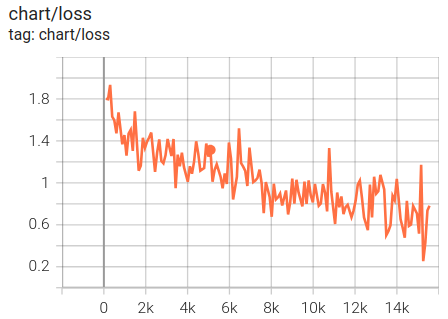
\includegraphics[width=0.32\textwidth]{../code/figures/1_loss.png}}
  \subfigure[训练中准确率图像]{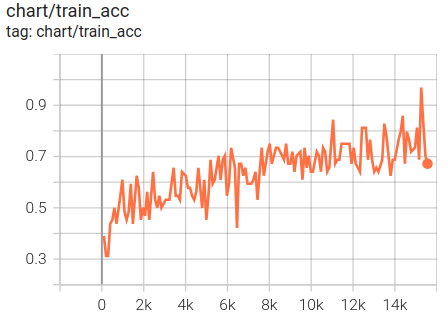
\includegraphics[width=0.32\textwidth]{../code/figures/1_train_acc.png}}
  \subfigure[训练中准确率图像]{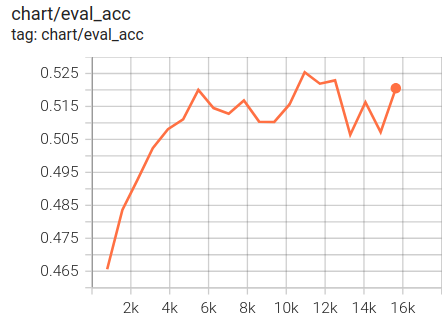
\includegraphics[width=0.32\textwidth]{../code/figures/1_eval_acc.png}}
  \setlength{\abovecaptionskip}{0ex}  % 如果使用了minted会增大图像与标题间距需要进行缩小
  \caption{训练20个epochs的TensorBoard日志图像,在验证集上的最优准确率为第11个epoch时的52.54\%}
  \label{fig-1}
\end{figure}
\subsection{在cifar10上用PyTorch训练卷积网络分类器}
与全连接神经网络不同之处在于:
\begin{enumerate}
    \item 使用了图像增强,包括随机裁剪,随机水平翻转,色彩抖动;
    \item 三个CNN卷积块(2D卷积,批归一化,Mish激活函数),每个卷积块后经过一个最大池化将图像缩小一倍,
    最后展平,用全连接做输出头预测类别。
\end{enumerate}
\begin{pythoncode}
import time
from pathlib import Path

import torch
import torch.nn as nn
import torch.optim as optim
from torchvision import datasets, transforms
from torch.utils.data import DataLoader
from torch.utils.tensorboard.writer import SummaryWriter

# Tensorbaord日志
path_log = Path(f"./logs/{time.strftime('%Y%m%d-%H%M%S')}")
writer = SummaryWriter(path_log)

# 检查是否有可用 GPU
device = torch.device("cuda" if torch.cuda.is_available() else "cpu")
print(f"Using device: {device}")

# 超参数设置
batch_size = 64
learning_rate = 0.001
num_epochs = 20

# 数据增强和预处理
transform_train = transforms.Compose([
  transforms.RandomCrop(32, padding=4),      # 随机裁剪
  transforms.RandomHorizontalFlip(),      # 随机水平翻转
  transforms.ColorJitter(brightness=0.2, contrast=0.2, saturation=0.2, hue=0.1),  # 色彩抖动
  transforms.ToTensor(),
  transforms.Normalize((0.5, 0.5, 0.5), (0.5, 0.5, 0.5))  # 标准化
])

transform_test = transforms.Compose([
  transforms.ToTensor(),
  transforms.Normalize((0.5, 0.5, 0.5), (0.5, 0.5, 0.5))
])

train_dataset = datasets.CIFAR10(root='./data', train=True, transform=transform_train, download=True)
test_dataset = datasets.CIFAR10(root='./data', train=False, transform=transform_test, download=True)

train_loader = DataLoader(train_dataset, batch_size=batch_size, shuffle=True)
test_loader = DataLoader(test_dataset, batch_size=batch_size, shuffle=False)

class CNN(nn.Module):
  def __init__(self, in_ch, out_ch, kernel, stride, padding):
    super().__init__()
    self.conv = nn.Conv2d(in_ch, out_ch, kernel_size=kernel, stride=stride, padding=padding)
    self.bn = nn.BatchNorm2d(out_ch)
    self.mish = nn.Mish()
  
  def forward(self, x):
    return self.mish(self.bn(self.conv(x)))

# 定义 CNN 模型
class Model(nn.Module):
  def __init__(self, num_classes=10):
    super().__init__()
    self.backbone = nn.Sequential(
      CNN(3, 64, 3, 1, 1),
      nn.MaxPool2d(kernel_size=2, stride=2),
      CNN(64, 128, 3, 1, 1),
      nn.MaxPool2d(kernel_size=2, stride=2),
      CNN(128, 256, 3, 1, 1),
      nn.MaxPool2d(kernel_size=2, stride=2),
    )
    self.head = nn.Sequential(
      nn.Linear(256 * 4 * 4, 512),
      nn.Mish(),
      nn.Linear(512, num_classes),
    )

  def forward(self, x):
    x = self.backbone(x)
    x = nn.Flatten()(x)
    x = self.head(x)
    return x

# 初始化模型、损失函数和优化器
model = Model().to(device)
criterion = nn.CrossEntropyLoss()
optimizer = optim.Adam(model.parameters(), lr=learning_rate)
global_step = 0
best_eval_acc = 0

# 训练模型
for epoch in range(num_epochs):
  model.train()
  for batch_idx, (data, target) in enumerate(train_loader):
    data, target = data.to(device), target.to(device)

    # 前向传播
    outputs = model(data)
    loss = criterion(outputs, target)
    _, predicted = torch.max(outputs, 1)
    acc = (target == predicted).sum().item() / batch_size

    # 反向传播
    optimizer.zero_grad()
    loss.backward()
    optimizer.step()
    global_step += 1

    if (batch_idx + 1) % 100 == 0:
      writer.add_scalar("chart/loss", loss.item(), global_step)
      writer.add_scalar("chart/train_acc", acc, global_step)
      print(f"Epoch [{epoch + 1}/{num_epochs}], Step [{batch_idx + 1}/{len(train_loader)}], Loss: {loss.item():.4f}, Acc: {acc:.4f}")

  # 测试模型
  model.eval()
  correct = 0
  total = 0
  with torch.no_grad():
    for data, target in test_loader:
      data, target = data.to(device), target.to(device)
      outputs = model(data)
      _, predicted = torch.max(outputs.data, 1)
      total += target.size(0)
      correct += (predicted == target).sum().item()

  eval_acc = correct / total
  print(f"Test Accuracy: {100 * eval_acc:.2f}%")
  writer.add_scalar("chart/eval_acc", eval_acc, global_step)

  if eval_acc > best_eval_acc:
    best_eval_acc = eval_acc
    # 保存最优eval模型
    path_save_model = f"cifar10_fc_model_best_eval.pth"
    torch.save(model.state_dict(), path_log / path_save_model)
    print(f"Best eval model ({100*eval_acc:.2f}%) saved as {path_log / path_save_model}")

# 保存模型
path_save_model = f"cifar10_fc_model_{global_step}.pth"
torch.save(model.state_dict(), path_log / path_save_model)
print(f"Last model saved as {path_log / path_save_model}")
print(f"Best eval accuracy {100 * best_eval_acc:.2f}%")
\end{pythoncode}
TensorBoard日志图片如下:
\begin{figure}[H]
  \centering
  \subfigure[损失函数图像]{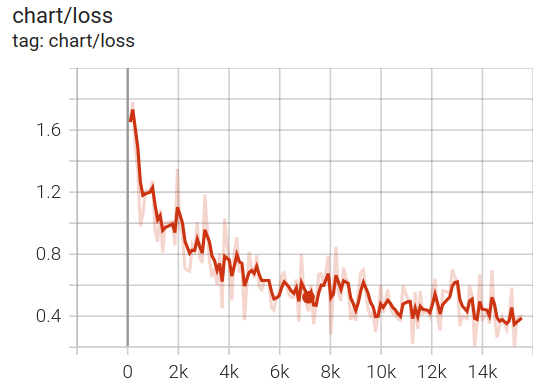
\includegraphics[width=0.32\textwidth]{../code/figures/2_loss.png}}
  \subfigure[训练中准确率图像]{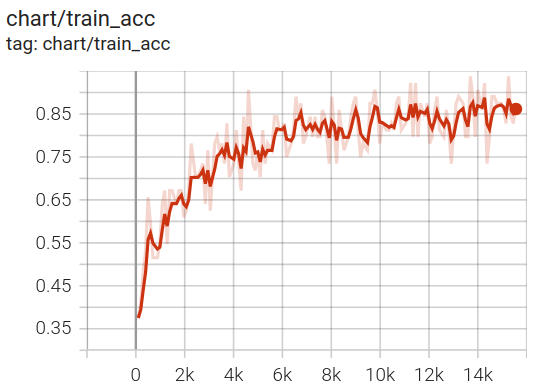
\includegraphics[width=0.32\textwidth]{../code/figures/2_train_acc.png}}
  \subfigure[训练中准确率图像]{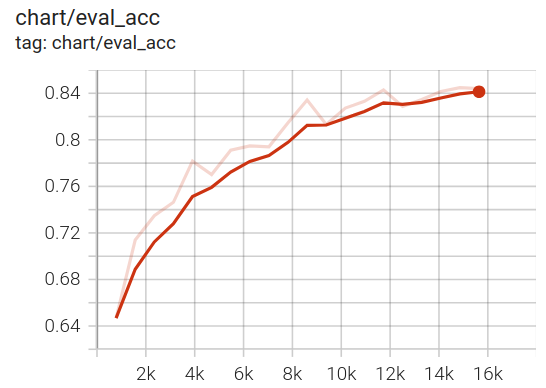
\includegraphics[width=0.32\textwidth]{../code/figures/2_eval_acc.png}}
  \setlength{\abovecaptionskip}{0ex}  % 如果使用了minted会增大图像与标题间距需要进行缩小
  \caption{训练20个epochs的TensorBoard日志图像,在验证集上的最优准确率为第19个epoch时的84.48\%}
  \label{fig-1}
\end{figure}

\end{document}
